\documentclass[11pt]{article}
\usepackage[utf8]{inputenc}
\usepackage[T1]{fontenc}
\usepackage{amsmath, bm}
\usepackage{float}
\usepackage{hyperref, tikz}
\usepackage{bm}
\usepackage{tikz}
\usepackage{caption}
\usepackage{subcaption}

\usetikzlibrary{calc}
\setcounter{secnumdepth}{0}
\DeclareMathOperator{\relu}{ReLU}
\DeclareMathOperator{\sign}{sign}
\begin{document}
\begin{center}
  \mbox{}\\[2.0cm]
  \textsc{\Huge Deep Learning}\\[1.0cm]
  \textsc{\Large Homework 1}\\[0.5cm]
\end{center}
\begin{flushleft}
  Group 71 members: \\[0.5cm]
  \begin{itemize}
  \item Luis Jose De Macedo Guevara (95621)
  \item Vincent Jakl (108529)
  \end{itemize}
\end{flushleft}

\section{Contributions of each member}
\begin{itemize}
    \item Luis Jose De Macedo Guevara (95621):
    \item Vincent Jakl (108529):
\end{itemize}
\pagebreak
\section{Question 1}
\subsection{1. a)}
The single perceptron was not the best choice for this task.
As can be seen in the figure below, the perceptron was not able to fit to the high dimensional data also with no sign of improvement.
With the 20 epochs, it ended up with a 0.3422 test accuracy which is slightly higher than 0.25 that would happen with random selection for 4 classes.
Also the learning rate was left at the value of 1 so this might cause the problem as well.
\begin{figure}[h!]
  \centering
  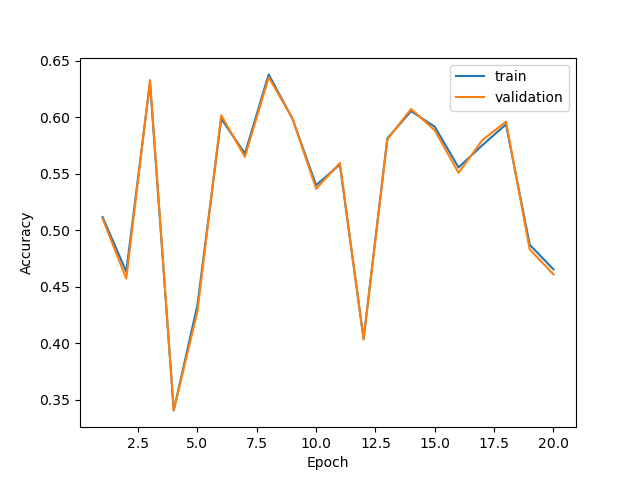
\includegraphics[width=0.5\textwidth]{./plots/single_perceptron.png}
  \caption{Single perceptron}\label{fig:single_layer_perceptron}
\end{figure}

\subsection{1. b)}
The logistic regression performed better than the single perceptron.
As can be seen in the figure below, the logistic regression was able to fit to the data better.
There was however a big difference between the two learning rates.
Where the model with the learning rate of 0.01 jumped faster to the higher accuracy, it did not improve on a regular basis.
The 0.001 lr model was a bit slower to get up to higher accuracy, but it was able to consistently improve.
In the end the 0.01 lr model ended up with 0.5784 test accuracy and the 0.001 lr model ended up with 0.5936 test accuracy.
Running these models for more epochs would possibly improve the accuracy since the trainig was still showing signs of improvement even with the evaluation metric.

\begin{figure}
\centering
\begin{subfigure}{.5\textwidth}
  \centering
  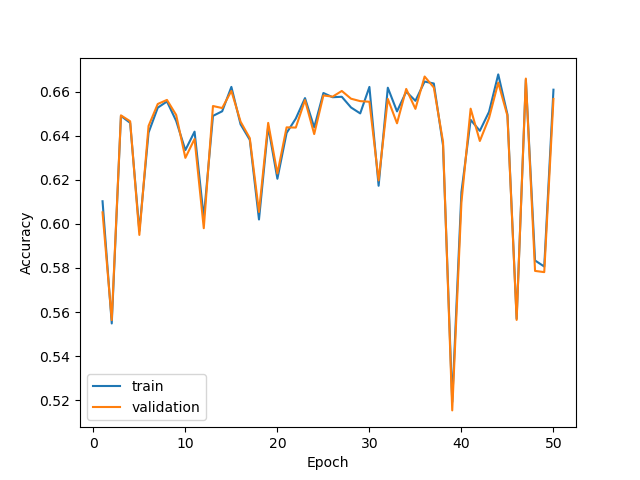
\includegraphics[width=.9\linewidth]{./plots/logistic_regression_0.01.png}
  \caption{lr 0.01}
  \label{fig:sub1}
\end{subfigure}%
\begin{subfigure}{.5\textwidth}
  \centering
  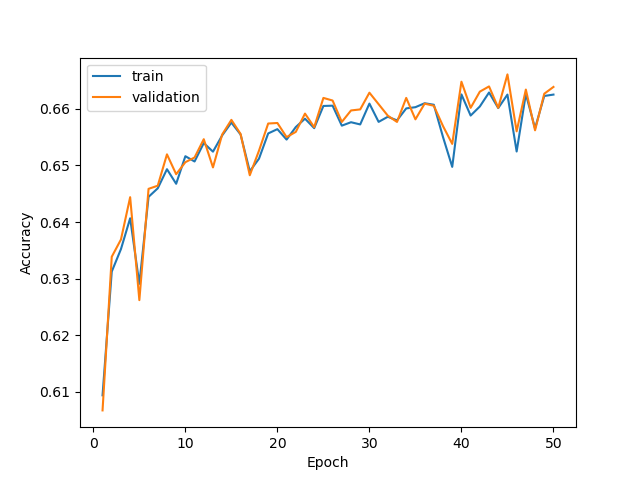
\includegraphics[width=.9\linewidth]{./plots/logistic_regression_0.001.png}
  \caption{lr 0.001}
  \label{fig:sub2}
\end{subfigure}
\caption{Logistic regression}
\label{fig:logistic_regression}
\end{figure}

\subsection{2. a)}
\subsection{2. b)}
\pagebreak
\section{Question 2}
\subsection{1.}
\subsection{2. a)}
\subsection{2. b)}
\subsection{2. c)}
\pagebreak
\section{Question 3}
\subsection{1.}
\subsubsection{a)}
Let
\begin{itemize}
  \item $D = 2$
  \item $A = B = 0$
  \item $\bm{x}^{(1)} = \begin{bmatrix} 1 \\ 1\end{bmatrix}$, $\bm{x}^{(2)} = \begin{bmatrix} 1 \\ -1\end{bmatrix}$, $\bm{x}^{(3)} = \begin{bmatrix} -1 \\ 1\end{bmatrix}$ and $\bm{x}^{(4)} = \begin{bmatrix} -1 \\ -1\end{bmatrix}$, 
  \end{itemize}
  We have $f ( \bm{x}^{(1)}) = -1$, $f ( \bm{x}^{(2)}) = +1$, $f ( \bm{x}^{(3)}) = +1$ and $f ( \bm{x}^{(4)}) = -1$

  \begin{figure}[h!]
  \begin{tikzpicture}[xscale=2, yscale=2, domain=0.140:60,samples=800]
    \draw[->] (-2, 0) -- (2, 0) node[right] {$x$};
    \draw[->] (0, -2) -- (0, 2) node[above] {$y$};
    \foreach \i in {-1, 1} {
        \draw (\i, 0.05) -- (\i, -0.05) node[below] {$\i$};
        \draw (0.05, \i) -- (-0.05, \i) node[left] {$\i$};
    }

    \node[red, scale=1.5] at (1, 1) {\textbullet};
    \node[green, scale=1.5] at (-1, 1) {\textbullet};
    \node[green, scale=1.5] at (1, -1) {\textbullet};
    \node[red, scale=1.5] at (-1, -1) {\textbullet};
  \end{tikzpicture}
  \end{figure}
  Which we can see is not linearly separable and therefore a perceptron cannot learn a separating hyperplane.
\pagebreak
\subsubsection{b)}
\begin{figure*}[h!]
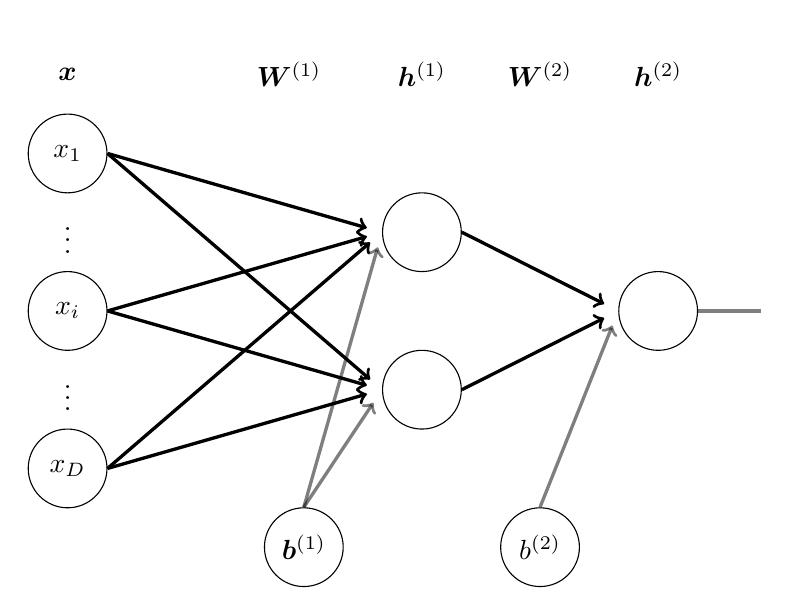
\begin{tikzpicture}
  \draw (0, 0) node[circle, minimum size=10mm, draw] (x1) {$x_{1}$};
  \draw ($(x1) - (0, 1)$) node[circle, minimum size=10mm] (xd1) {$\vdots$};
  \draw ($(xd1) - (0, 1)$) node[circle, minimum size=10mm, draw] (xi) {$x_{i}$};
  \draw ($(xi) - (0, 1)$) node[circle, minimum size=10mm] (xd2) {$\vdots$};
  \draw ($(xd2) - (0, 1)$) node[circle, minimum size=10mm, draw] (xD) {$x_{D}$};

  \draw ($(x1.north) + (0, 0.5)$) node[circle, minimum size=10mm] (x) {$\bm{x}$};
% h^(1)
  \foreach \i in{1, 2}{
    \draw ($(xd\i) + (4.5, 0)$) node[circle, minimum size=10mm, draw] (h1\i) {};
    \foreach \j in {1, i, D}{
      \draw[very thick, ->, shorten >=2mm] (x\j.east) -- (h1\i.west);
    }
  }
  \draw ($(h11.north) + (0, 1.5)$) node[circle, minimum size=10mm] (h1) {$\bm{h}^{(1)}$};

  \draw ($(h12) - (1.5, 2)$) node[circle, minimum size=10mm, draw] (b1) {$\bm{b}^{(1)}$};

  \foreach \i in {1, 2}{
    \draw[very thick, ->, shorten >=2mm, opacity=0.5] (b1.north) -- (h1\i.west);
  }

% h^(2)
  \draw ($(h12) + (3, 1)$) node[circle, minimum size=10mm, draw] (h21) {};
  \foreach \j in {1, 2}{
    \draw[very thick, ->, shorten >=2mm] (h1\j.east) -- (h21.west);
  }
  \draw ($(h21.north) + (0, 2.5)$) node[circle, minimum size=10mm] (h2) {$\bm{h}^{(2)}$};

  \draw ($(h21) - (1.5, 3)$) node[circle, minimum size=10mm, draw] (b2) {$b^{(2)}$};

  \draw[very thick, ->, shorten >=2mm, opacity=0.5] (b2.north) -- (h21.west);

  \draw ($(h1)!0.375!(x)$) node[circle, minimum size=10mm] {$\bm{W}^{(1)}$};
  \draw ($(h1)!0.5!(h2)$) node[circle, minimum size=10mm] {$\bm{W}^{(2)}$};

  \draw[very thick, shorten >=2mm, opacity=0.5] (h21.east) -- ++(1, 0);
\end{tikzpicture}
\end{figure*}
\begin{align*}
  \bm{W}^{(1)} &= \underbrace{\begin{bmatrix}
                   1  &1  &\cdots &1 \\
                   -1 &-1 &\cdots &-1
                 \end{bmatrix}}_{2 \times D}, &\bm{b}^{(1)} &= \begin{bmatrix}
                                                  -A \\
                                                  B
                                                 \end{bmatrix} \\
  \bm{W}^{(2)} &= \begin{bmatrix}
                   1 & 1
                 \end{bmatrix}, &\quad b^{(2)} &= -1
\end{align*}
We have for $\bm{x}$:
\begin{align*}
  \bm{h}^{(2)} &= \sign \left( \bm{W}^{(2)}\bm{h}^{(1)} + b^{(2)} \right) \\
               &= \sign \left( \bm{W}^{(2)} \left( \sign \left( \bm{W}^{(1)} \bm{x} + \bm{b}^{(1)} \right) \right) + b^{(2)} \right) \\
               &= \sign \left( \begin{bmatrix}
                                       1  &1
                                     \end{bmatrix} \left( \sign \left( \begin{bmatrix}
                                                                               1  &1  &\cdots &1 \\
                                                                               -1 &-1 &\cdots &-1
                                                                             \end{bmatrix}
                 \begin{bmatrix}
                   x_{1} \\
                   x_{2} \\
                   \vdots \\
                   x_{D}
                 \end{bmatrix} + \begin{bmatrix}
                                   -A \\
                                   B
                                 \end{bmatrix} \right) \right) -1 \right) \\
               &= \sign \left( \begin{bmatrix}
                                       1  &1
                                     \end{bmatrix} \begin{bmatrix}
                                                                               \sign \left( \sum_{i = 1}^{D} x_{i} - A \right) \\
                                                                               \sign \left( B - \sum_{i = 1}^{D} x_{i} \right)
                                                          \end{bmatrix} -1 \right) \\
               &= \sign \left( \sign \left( \sum_{i = 1}^{D} x_{i} - A \right) + \sign \left( B - \sum_{i = 1}^{D} x_{i} \right) -1 \right)
\end{align*}
\subsubsection{c)}
\begin{figure*}[h!]
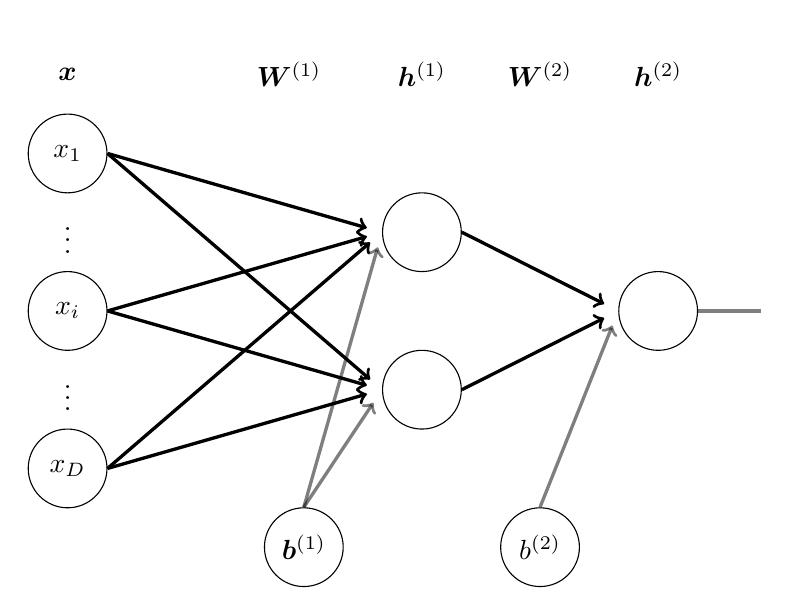
\begin{tikzpicture}
  \draw (0, 0) node[circle, minimum size=10mm, draw] (x1) {$x_{1}$};
  \draw ($(x1) - (0, 1)$) node[circle, minimum size=10mm] (xd1) {$\vdots$};
  \draw ($(xd1) - (0, 1)$) node[circle, minimum size=10mm, draw] (xi) {$x_{i}$};
  \draw ($(xi) - (0, 1)$) node[circle, minimum size=10mm] (xd2) {$\vdots$};
  \draw ($(xd2) - (0, 1)$) node[circle, minimum size=10mm, draw] (xD) {$x_{D}$};

  \draw ($(x1.north) + (0, 0.5)$) node[circle, minimum size=10mm] (x) {$\bm{x}$};
% h^(1)
  \foreach \i in{1, 2}{
    \draw ($(xd\i) + (4.5, 0)$) node[circle, minimum size=10mm, draw] (h1\i) {};
    \foreach \j in {1, i, D}{
      \draw[very thick, ->, shorten >=2mm] (x\j.east) -- (h1\i.west);
    }
  }
  \draw ($(h11.north) + (0, 1.5)$) node[circle, minimum size=10mm] (h1) {$\bm{h}^{(1)}$};

  \draw ($(h12) - (1.5, 2)$) node[circle, minimum size=10mm, draw] (b1) {$\bm{b}^{(1)}$};

  \foreach \i in {1, 2}{
    \draw[very thick, ->, shorten >=2mm, opacity=0.5] (b1.north) -- (h1\i.west);
  }

% h^(2)
  \draw ($(h12) + (3, 1)$) node[circle, minimum size=10mm, draw] (h21) {};
  \foreach \j in {1, 2}{
    \draw[very thick, ->, shorten >=2mm] (h1\j.east) -- (h21.west);
  }
  \draw ($(h21.north) + (0, 2.5)$) node[circle, minimum size=10mm] (h2) {$\bm{h}^{(2)}$};

  \draw ($(h21) - (1.5, 3)$) node[circle, minimum size=10mm, draw] (b2) {$b^{(2)}$};

  \draw[very thick, ->, shorten >=2mm, opacity=0.5] (b2.north) -- (h21.west);

  \draw ($(h1)!0.375!(x)$) node[circle, minimum size=10mm] {$\bm{W}^{(1)}$};
  \draw ($(h1)!0.5!(h2)$) node[circle, minimum size=10mm] {$\bm{W}^{(2)}$};

  \draw[very thick, shorten >=2mm, opacity=0.5] (h21.east) -- ++(1, 0);
\end{tikzpicture}
\end{figure*}
\begin{align*}
  \bm{W}^{(1)} &= \underbrace{\begin{bmatrix}
                   -1  &-1  &\cdots &-1 \\
                   1 &1 &\cdots &1
                 \end{bmatrix}}_{2 \times D}, &\bm{b}^{(1)} &= \begin{bmatrix}
                                                  A \\
                                                  -B
                                                 \end{bmatrix} \\
  \bm{W}^{(2)} &= \begin{bmatrix}
                   -1 & -1
                 \end{bmatrix}, &\quad b^{(2)} &= 0
\end{align*}
We have for $\bm{x}$:
\begin{align*}
  \bm{h}^{(2)} &= \sign \left( \bm{W}^{(2)}\bm{h}^{(1)} + b^{(2)} \right) \\
               &= \sign \left( \bm{W}^{(2)} \left( \relu \left( \bm{W}^{(1)} \bm{x} + \bm{b}^{(1)} \right) \right) + b^{(2)} \right) \\
               &= \sign \left( \begin{bmatrix}
                                       -1  &-1
                               \end{bmatrix} \left( \relu \left( \begin{bmatrix}
                                                                               -1  &-1  &\cdots &-1 \\
                                                                               1 &1 &\cdots &1
                                                                             \end{bmatrix}
                 \begin{bmatrix}
                   x_{1} \\
                   x_{2} \\
                   \vdots \\
                   x_{D}
                 \end{bmatrix} + \begin{bmatrix}
                                   A \\
                                   -B
                                 \end{bmatrix} \right) \right) \right) \\
               &= \sign \left( \begin{bmatrix}
                                       -1  &-1
                                     \end{bmatrix} \begin{bmatrix}
                                                     \relu \left( A - \sum_{i = 1}^{D} x_{i} \right) \\
                                                     \relu \left( \sum_{i = 1}^{D} x_{i} - B \right)
                                                   \end{bmatrix} \right) \\
               &= \sign \left( - \relu \left( A - \sum_{i = 1}^{D} x_{i} \right) - \relu \left( \sum_{i = 1}^{D} x_{i}  - B \right) \right)
\end{align*}
\end{document}